\chapter{Overview}

Zubax Komar is a high-quality FOC ESC based on the \text{T\'elega} motor control technology. Komar is designed 
to support the propulsion systems of light unmanned aerial vehicles (UAVs), unmanned underwater vehicles (UUVs) and
unmanned surface vehicles (USVs).

The controller provides up to 2500\,W of continuous power output\footnote{When forced air cooling is applied} and
supports a wide range of operating voltages: 13 -- 51\,V (4 -- 12S $\text{LiCoO}_\text{2}$ battery).
Komar is capable of being finely tuned to any motor-propellor combination for optimal dynamic responses.

Komar offers several control modes that make it suitable for a wide range of propulsion systems.
It is fully UAVCAN-compatible and can be easily integrated into an end system using the two standard UAVCAN
Micro connectors\footnote{For more details refer to
\url{https://uavcan.org/Specification/8._Hardware_design_recommendations/}} on each CAN interface.

Ensuring high levels of system reliability, Komar continuously measures and reports on all the critical
performance parameters including the controller temperature, the motor temperature, the instantaneous
DC link voltage and instantaneous DC link current.

\section{System integration}
Zubax Komar is a single-supply device that dedicates power to the motor. It does not expose any power supply
inputs to its internal components and the 5\,V rails of the CAN interfaces cannot be used by the controller
itself. Komar does, however, offer a power delivery feature that when enabled will deliver 5\,V to the power
distribution network.

\begin{figure}[h]
    \centering
    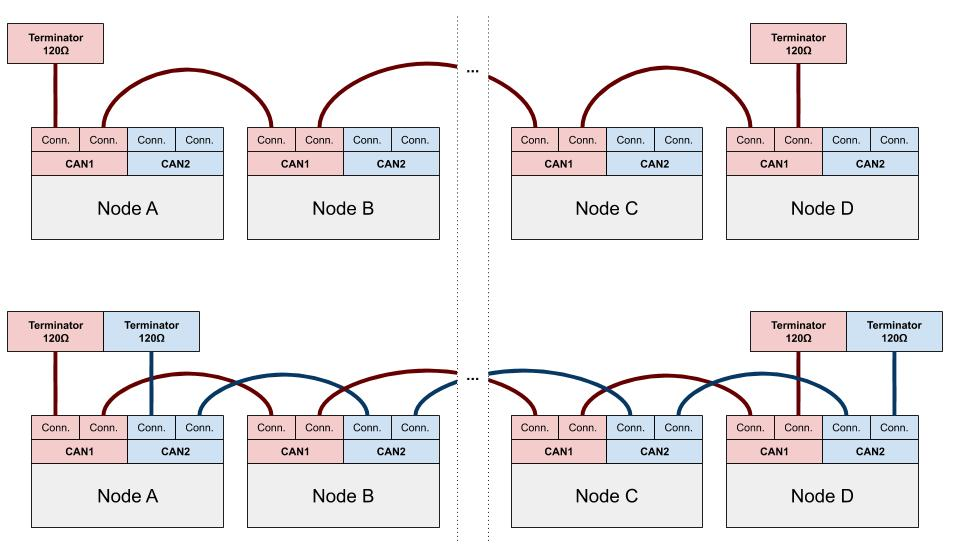
\includegraphics[width=1\textwidth]{can_integration.jpg}
    \caption{Connection of CAN nodes}
\end{figure}
